\documentclass[8pt,aspectratio=169]{beamer}
\usetheme{Madrid}
\usepackage{graphicx}
\usepackage{booktabs}
\usepackage{adjustbox}
\usepackage{multicol}
\usepackage{amsmath}
\usepackage{amssymb}
\usepackage{tcolorbox}
\usepackage{xcolor}
\usepackage{tikz}
\usetikzlibrary{shapes.geometric, arrows, positioning}
\usepackage{listings}

% Define colors matching the ML Design course theme
\definecolor{mlblue}{RGB}{31, 119, 180}
\definecolor{mlorange}{RGB}{255, 127, 14}
\definecolor{mlgreen}{RGB}{44, 160, 44}
\definecolor{mlred}{RGB}{214, 39, 40}
\definecolor{mlpurple}{RGB}{148, 103, 189}
\definecolor{mlbrown}{RGB}{140, 86, 75}
\definecolor{mlpink}{RGB}{227, 119, 194}
\definecolor{mlgray}{RGB}{127, 127, 127}
\definecolor{mlyellow}{RGB}{255, 187, 120}
\definecolor{mlcyan}{RGB}{23, 190, 207}

% Remove navigation symbols and add custom footer
\setbeamertemplate{navigation symbols}{}
\setbeamertemplate{footline}{
  \leavevmode%
  \hbox{%
  \begin{beamercolorbox}[wd=.25\paperwidth,ht=2.25ex,dp=1ex,center]{author in head/foot}%
    \usebeamerfont{author in head/foot}Week 2
  \end{beamercolorbox}%
  \begin{beamercolorbox}[wd=.5\paperwidth,ht=2.25ex,dp=1ex,center]{title in head/foot}%
    \usebeamerfont{title in head/foot}Clustering for Deep Empathy
  \end{beamercolorbox}%
  \begin{beamercolorbox}[wd=.25\paperwidth,ht=2.25ex,dp=1ex,right]{date in head/foot}%
    \usebeamerfont{date in head/foot}\insertframenumber{} / \inserttotalframenumber\hspace*{2ex} 
  \end{beamercolorbox}}%
  \vskip0pt%
}

% Code listing settings for syntax highlighting
\lstset{
    language=Python,
    basicstyle=\small\ttfamily,
    numbers=left,
    numberstyle=\tiny\color{gray},
    stepnumber=1,
    numbersep=5pt,
    backgroundcolor=\color{gray!5},
    showspaces=false,
    showstringspaces=false,
    showtabs=false,
    frame=single,
    rulecolor=\color{gray!30},
    tabsize=2,
    captionpos=b,
    breaklines=true,
    breakatwhitespace=false,
    keywordstyle=\color{mlblue},
    commentstyle=\color{mlgreen},
    stringstyle=\color{mlorange}
}

% Reduce margins for more content space
\setbeamersize{text margin left=5mm,text margin right=5mm}

% Title information
\title{\Large\textbf{Machine Learning for Smarter Innovation}}
\subtitle{\Large Week 2: Clustering for Deep Empathy}
\author{BSc Course in AI-Enhanced Innovation}
\institute{Understanding Users Through Data-Driven Segmentation}
\date{}

\begin{document}

% Title slide
\begin{frame}[plain]
\titlepage
\end{frame}

% Table of contents
\begin{frame}{Today's Journey: From Data to Deep Understanding}
\tableofcontents
\vfill
\begin{center}
\Large\textcolor{mlpurple}{\textbf{Transform data points into human insights}}
\end{center}
\end{frame}

% Include all parts
% Part 1: Foundation - Language & Emotion
\section{Foundation: Language as Window to Emotion}

% Slide 1: Opening Power Chart - Emotion Spectrum Heatmap
\begin{frame}[plain]
\centering
\includegraphics[width=0.85\textwidth]{charts/emotion_spectrum_heatmap.pdf}
\end{frame}

% Slide 2: The Power of Understanding Emotion
\begin{frame}{The Power of Understanding Emotion}
\Large\textbf{Why Language Reveals What Users Really Feel}
\normalsize

\vspace{0.5em}

\begin{columns}[T]
\begin{column}{0.48\textwidth}
\textbf{Traditional Analysis}
\begin{itemize}
\item Keyword counting
\item Manual categorization
\item Surface-level insights
\item Limited scale
\item Misses context
\end{itemize}
\end{column}
\begin{column}{0.48\textwidth}
\textbf{NLP-Powered Analysis}
\begin{itemize}
\item Contextual understanding
\item Emotion detection
\item Sarcasm recognition
\item Unlimited scale
\item Deep insights
\end{itemize}
\end{column}
\end{columns}

\vspace{1em}
\begin{tcolorbox}[colback=mlblue!10,colframe=mlblue]
\centering
``I love waiting 2 hours for support!'' $\rightarrow$ Negative (sarcasm detected)
\end{tcolorbox}
\end{frame}

% Slide 3: Language as Window to Emotion
\begin{frame}{Language as Window to User Experience}
\Large\textbf{Every Word Tells a Story}
\normalsize

\begin{columns}[T]
\begin{column}{0.55\textwidth}
\includegraphics[width=0.85\textwidth]{charts/language_emotion_flow.pdf}
\end{column}
\begin{column}{0.43\textwidth}
\textbf{What Language Reveals:}
\begin{itemize}
\item Frustration points
\item Delight moments
\item Unmet expectations
\item Hidden needs
\item Emotional journey
\end{itemize}

\vspace{0.5em}
\textbf{Design Insights:}
\begin{itemize}
\item Priority pain points
\item Feature requests
\item User segments
\item Experience gaps
\end{itemize}
\end{column}
\end{columns}
\end{frame}

% Slide 4: Beyond Keywords - Context Matters
\begin{frame}{Beyond Keywords: Context is Everything}
\Large\textbf{Same Words, Different Meanings}
\normalsize

\begin{center}
\includegraphics[width=0.75\textwidth]{charts/context_sentiment_examples.pdf}
\end{center}

\begin{columns}[T]
\begin{column}{0.32\textwidth}
\textbf{``This is sick!''}
\begin{itemize}
\small
\item Gaming: Positive
\item Healthcare: Negative
\item Teen slang: Positive
\end{itemize}
\end{column}
\begin{column}{0.32\textwidth}
\textbf{``It's fine''}
\begin{itemize}
\small
\item After complaint: Negative
\item First try: Neutral
\item With ``!'': Positive
\end{itemize}
\end{column}
\begin{column}{0.32\textwidth}
\textbf{``Interesting...''}
\begin{itemize}
\small
\item Academic: Positive
\item In review: Neutral
\item With ``...'': Skeptical
\end{itemize}
\end{column}
\end{columns}
\end{frame}

% Slide 5: Sentiment vs Emotion Analysis
\begin{frame}{Sentiment vs Emotion: Different Lenses}
\Large\textbf{From Polarity to Emotional Spectrum}
\normalsize

\begin{columns}[T]
\begin{column}{0.48\textwidth}
\textbf{Sentiment Analysis}
\begin{itemize}
\item Positive / Negative / Neutral
\item Overall polarity
\item Simple classification
\item Good for trends
\end{itemize}

\vspace{0.5em}
\includegraphics[width=0.85\textwidth]{charts/sentiment_distribution.pdf}
\end{column}
\begin{column}{0.48\textwidth}
\textbf{Emotion Analysis}
\begin{itemize}
\item Joy, Anger, Fear, Sadness, Surprise...
\item Nuanced understanding
\item Multi-class detection
\item Better for design
\end{itemize}

\vspace{0.5em}
\includegraphics[width=0.85\textwidth]{charts/emotion_wheel.pdf}
\end{column}
\end{columns}
\end{frame}

% Slide 6: The NLP Challenge in Design
\begin{frame}{The NLP Challenge: Scale Meets Nuance}
\Large\textbf{Processing Millions While Preserving Meaning}
\normalsize

\begin{center}
\includegraphics[width=0.85\textwidth]{charts/nlp_challenge_pyramid.pdf}
\end{center}

\begin{columns}[T]
\begin{column}{0.48\textwidth}
\textbf{Volume Challenges:}
\begin{itemize}
\item Thousands of reviews daily
\item Multiple languages
\item Various platforms
\item Real-time processing
\end{itemize}
\end{column}
\begin{column}{0.48\textwidth}
\textbf{Nuance Challenges:}
\begin{itemize}
\item Cultural context
\item Domain specificity
\item Evolving language
\item Individual expression
\end{itemize}
\end{column}
\end{columns}
\end{frame}

% Slide 7: Learning Objectives
\begin{frame}{Week 3 Learning Objectives}
\Large\textbf{What You'll Master}
\normalsize

\begin{columns}[T]
\begin{column}{0.48\textwidth}
\textbf{Technical Skills}
\begin{itemize}
\item Text preprocessing pipelines
\item BERT and transformers
\item Sentiment classification
\item Emotion detection
\item Aspect-based analysis
\item Model evaluation
\end{itemize}
\end{column}
\begin{column}{0.48\textwidth}
\textbf{Design Applications}
\begin{itemize}
\item Voice of Customer analysis
\item Emotional journey mapping
\item Pain point identification
\item Feature prioritization
\item Persona refinement
\item Experience optimization
\end{itemize}
\end{column}
\end{columns}

\vspace{1em}
\begin{tcolorbox}[colback=mlgreen!10,colframe=mlgreen]
\centering
\textbf{Outcome:} Transform text into actionable design insights at scale
\end{tcolorbox}
\end{frame}

% Slide 8: Real-world Impact
\begin{frame}{Real-world Impact: NLP in Action}
\Large\textbf{Companies Using NLP for Better Design}
\normalsize

\begin{columns}[T]
\begin{column}{0.32\textwidth}
\textbf{Airbnb}
\begin{itemize}
\small
\item Review analysis
\item Experience gaps
\item Host coaching
\item 23\% better ratings
\end{itemize}
\end{column}
\begin{column}{0.32\textwidth}
\textbf{Spotify}
\begin{itemize}
\small
\item Mood detection
\item Playlist curation
\item User feedback
\item 40\% more engagement
\end{itemize}
\end{column}
\begin{column}{0.32\textwidth}
\textbf{Slack}
\begin{itemize}
\small
\item Support tickets
\item Feature requests
\item User frustration
\item 50\% faster resolution
\end{itemize}
\end{column}
\end{columns}

\vspace{1em}
\begin{center}
\includegraphics[width=0.7\textwidth]{charts/nlp_impact_metrics.pdf}
\end{center}
\end{frame}
% PART 2 SECTION DIVIDER
\begin{frame}[plain]
\begin{center}
\vspace{2em}
\Large\textcolor{mlgreen}{\textbf{PART 2}}\\
\vspace{0.5em}
\Large\textbf{Technical Core}\\
\vspace{2em}
\Large
What we'll learn:\\
\vspace{1em}
\normalsize
\begin{itemize}
\item K-means clustering algorithm
\item Finding optimal K with elbow method
\item Distance metrics and quality measures
\item Advanced techniques (DBSCAN, Hierarchical)
\item Feature importance analysis
\end{itemize}
\vspace{2em}
\Large\textcolor{mlpurple}{\textbf{Learning the basics step by step}}
\end{center}
\end{frame}

% Learning Objectives for Part 2
\begin{frame}
\frametitle{\Large Part 2: Learning Objectives}
\framesubtitle{Technical Skills You'll Develop}

\begin{columns}[T]
\begin{column}{0.48\textwidth}
\begin{tcolorbox}[colback=mlgreen!10, colframe=mlgreen!50, title={By the end of Part 2, you will understand:}]
\normalsize
\begin{itemize}
\item \textbf{How} K-means clustering works
\item \textbf{What} the elbow method shows us
\item \textbf{Why} we measure distances
\item \textbf{How to check} if clusters are good
\item \textbf{Differences} between algorithms
\item \textbf{When to use} each method
\end{itemize}
\end{tcolorbox}
\end{column}

\begin{column}{0.48\textwidth}
\begin{tcolorbox}[colback=mlorange!10, colframe=mlorange!50, title=Practical Skills]
\normalsize
\begin{itemize}
\item Use K-means step by step
\item Understand quality scores
\item Pick the right algorithm
\item Adjust settings properly
\item Work with different patterns
\item Prepare data for analysis
\end{itemize}
\end{tcolorbox}
\end{column}
\end{columns}
\end{frame}

% PART 2: TECHNICAL CORE (10 slides)

% Section Divider: Part 2
\begin{frame}
\begin{center}
\vspace{2cm}
{\Huge\textbf{PART 2}}

\vspace{0.5cm}
{\LARGE Technical Core}

\vspace{1cm}
{\large Machine Learning Algorithms \& Implementation}
\end{center}
\end{frame}

% THE CLUSTERING PROBLEM
\begin{frame}
\frametitle{\Large The Innovation Classification Problem}
\framesubtitle{5000 Ideas - How Do They Connect?}

\begin{columns}[T]
\begin{column}{0.48\textwidth}
\begin{tcolorbox}[colback=mlred!10, colframe=mlred!50, title=The Pain]
\textbf{Current Reality:}
\begin{itemize}
\item One-size-fits-all solutions
\item Generic innovation categories
\item Missed opportunities
\item Unhappy edge cases
\end{itemize}
\vspace{0.5em}
\textbf{The Cost:}
\begin{itemize}
\item Most innovations get misclassified
\item Features with low adoption rates
\item Inefficient resource allocation
\end{itemize}
\end{tcolorbox}
\end{column}

\begin{column}{0.48\textwidth}
\begin{tcolorbox}[colback=mlgreen!10, colframe=mlgreen!50, title=The Question]
\Large\textbf{What if we could...}
\normalsize
\begin{itemize}
\item Find natural innovation clusters?
\item Discover innovation patterns?
\item Innovate at scale?
\item Identify opportunity gaps?
\end{itemize}
\vspace{0.5em}
\Large\textcolor{mlpurple}{\textbf{We can!}}\\
\normalsize\textbf{Solution: Clustering}
\end{tcolorbox}
\end{column}
\end{columns}
\end{frame}

% NEW: Current Reality Visualization
\begin{frame}
\frametitle{\Large Current Reality: The Problem}
\framesubtitle{Why One-Size-Fits-All Doesn't Work}

\begin{center}
\includegraphics[width=0.85\textwidth]{charts/current_reality_visual.pdf}
\end{center}
\end{frame}

% NEW: Innovation Archetypes Definition
\begin{frame}
\frametitle{\Large Innovation Archetypes}
\framesubtitle{Common Patterns We'll Discover}

\begin{columns}[T]
\begin{column}{0.48\textwidth}
\textbf{\large Core Innovation Types}
\vspace{0.5em}

\textcolor{mlred}{\textbf{Disruptive Innovation}}\\
Completely new approaches that reshape markets

\vspace{0.5em}
\textcolor{mlblue}{\textbf{Incremental Innovation}}\\
Step-by-step improvements to existing solutions

\vspace{0.5em}
\textcolor{mlgreen}{\textbf{Service Innovation}}\\
New ways to deliver value to customers
\end{column}

\begin{column}{0.48\textwidth}
\textbf{\large Emerging Patterns}
\vspace{0.5em}

\textcolor{mlorange}{\textbf{Business Model Innovation}}\\
New ways to create and capture value

\vspace{0.5em}
\textcolor{mlpurple}{\textbf{Process Innovation}}\\
Better ways to produce and deliver

\vspace{0.5em}
\textcolor{mlpink}{\textbf{Platform Innovation}}\\
Creating ecosystems for innovation
\end{column}
\end{columns}

\vspace{0.5em}
\begin{center}
\large\textcolor{mlpurple}{\textbf{Clustering will reveal which type each idea belongs to}}
\end{center}
\end{frame}

% Slide 9: What is Clustering?
\begin{frame}
\frametitle{\Large What is Clustering?}
\framesubtitle{Like Organizing a Messy Room - Finding Things That Belong Together}

\begin{center}
\includegraphics[width=0.75\textwidth]{charts/chaos_to_clarity.pdf}
\end{center}

\vspace{0.5em}
\begin{columns}[T]
\begin{column}{0.48\textwidth}
\Large\textbf{Clustering Finds:}
\normalsize
\begin{itemize}
\item Natural groupings
\item Similar approaches  
\item Hidden patterns
\item Innovation relationships
\end{itemize}
\end{column}

\begin{column}{0.48\textwidth}
\begin{tcolorbox}[colback=mlgreen!10, colframe=mlgreen!50]
\textbf{Key Insight:}\\
Things that look similar often belong in the same group\\
\textit{(Just like organizing books by topic on a shelf)}
\end{tcolorbox}
\end{column}
\end{columns}
\end{frame}

% Slide 10: K-Means Algorithm Part 1
\begin{frame}
\frametitle{\Large K-Means: The Basic Clustering Method (Part 1)}
\framesubtitle{Initial Setup - Like Choosing City Centers}

\begin{columns}[T]
\begin{column}{0.48\textwidth}
\Large\textbf{Steps 1-2: Setup}
\normalsize
\vspace{0.5em}

\textbf{Step 1: Choose K}
\begin{itemize}
\item Decide number of clusters
\item Based on domain knowledge
\item Or use elbow method
\end{itemize}

\vspace{0.5em}
\textbf{Step 2: Initialize Centroids}
\begin{itemize}
\item Place K random points
\item These are initial cluster centers
\item Random but spread out
\end{itemize}

\vspace{0.5em}
\textcolor{mlblue}{\textbf{Key Decision: How many groups make sense?}}
\end{column}

\begin{column}{0.48\textwidth}
\begin{center}
\includegraphics[width=\textwidth]{charts/kmeans_animation.pdf}
\end{center}
\textit{Visualization: Initial random centroids placed}
\end{column}
\end{columns}
\end{frame}

% Slide 11: K-Means Algorithm Part 2
\begin{frame}
\frametitle{\Large K-Means: The Basic Clustering Method (Part 2)}
\framesubtitle{Iteration Process - Finding Natural Groups}

\begin{columns}[T]
\begin{column}{0.48\textwidth}
\Large\textbf{Steps 3-5: Iterate}
\normalsize
\vspace{0.5em}

\textbf{Step 3: Assign Points}
\begin{itemize}
\item Calculate distance to each centroid
\item Assign to nearest centroid
\item Forms initial clusters
\end{itemize}

\vspace{0.5em}
\textbf{Step 4: Update Centroids}
\begin{itemize}
\item Calculate mean of each cluster
\item Move centroid to that mean
\item Centers shift to better positions
\end{itemize}

\vspace{0.5em}
\textbf{Step 5: Check Convergence}
\begin{itemize}
\item Repeat steps 3-4
\item Stop when centroids don't move
\item Usually 5-10 iterations
\end{itemize}
\end{column}

\begin{column}{0.48\textwidth}
\begin{center}
\includegraphics[width=\textwidth]{charts/kmeans_animation.pdf}
\end{center}
\textit{Iteration 1 $\rightarrow$ 3 $\rightarrow$ 5 $\rightarrow$ \textbf{Converged}}
\end{column}
\end{columns}
\end{frame}

% PROBLEM: HOW MANY GROUPS?
\begin{frame}
\frametitle{\Large The Goldilocks Problem}
\framesubtitle{Too Few vs. Too Many Groups}

\begin{columns}[T]
\begin{column}{0.32\textwidth}
\begin{tcolorbox}[colback=mlred!10, colframe=mlred!50, title={Too Few (K=2)}]
\begin{center}
\textbf{Oversimplification}
\end{center}
\begin{itemize}
\normalsize
\item Mixed segments
\item Lost nuance
\item Generic solutions
\end{itemize}
\end{tcolorbox}
\end{column}

\begin{column}{0.32\textwidth}
\begin{tcolorbox}[colback=mlgreen!10, colframe=mlgreen!50, title=Just Right (K=5)]
\begin{center}
\textbf{Optimal Balance}
\end{center}
\begin{itemize}
\normalsize
\item Clear segments
\item Actionable insights
\item Manageable complexity
\end{itemize}
\end{tcolorbox}
\end{column}

\begin{column}{0.32\textwidth}
\begin{tcolorbox}[colback=mlorange!10, colframe=mlorange!50, title=Too Many (K=20)]
\begin{center}
\textbf{Analysis Paralysis}
\end{center}
\begin{itemize}
\normalsize
\item Overfitting
\item Tiny segments
\item Impossible to act on
\end{itemize}
\end{tcolorbox}
\end{column}
\end{columns}

\vspace{1em}
\begin{center}
\Large\textcolor{mlpurple}{\textbf{How do we find the sweet spot?}}
\end{center}
\end{frame}

% Slide 12: Choosing K - Elbow Method
\begin{frame}
\frametitle{\Large The Elbow Method}
\framesubtitle{How Many Groups Should We Have? (Like Goldilocks - Not Too Few, Not Too Many)}

\begin{columns}[T]
\begin{column}{0.43\textwidth}
\Large\textbf{Finding the Elbow:}
\normalsize
\begin{itemize}
\item Plot inertia vs K
\item Look for the ``elbow''
\item Balance between:
    \begin{itemize}
    \normalsize
    \item Too few: Mixed groups
    \item Too many: Overfitting
    \end{itemize}
\end{itemize}

\vspace{0.5em}
\begin{tcolorbox}[colback=mlblue!10, colframe=mlblue!50]
\textbf{Optimal K = 5}\\
Best trade-off between simplicity and accuracy
\end{tcolorbox}
\end{column}

\begin{column}{0.55\textwidth}
\begin{center}
\includegraphics[width=\textwidth]{charts/elbow_method.pdf}
\end{center}
\end{column}
\end{columns}
\end{frame}

% Slide 13: Distance Metrics
\begin{frame}
\frametitle{\Large Distance Metrics}
\framesubtitle{Different Ways to Measure "How Close" Things Are}

\begin{center}
\includegraphics[width=0.9\textwidth]{charts/distance_metrics_detailed.pdf}
\end{center}

\vspace{0.5em}
\begin{center}
\large\textcolor{mlpurple}{\textbf{Each metric reveals different patterns in your data}}
\end{center}
\end{frame}

% Slide 14: Cluster Quality
\begin{frame}
\frametitle{\Large Cluster Quality Metrics}
\framesubtitle{Are Our Groups Any Good? (Like Checking Your Work)}

\begin{center}
\includegraphics[width=0.75\textwidth]{charts/cluster_quality.pdf}
\end{center}

\vspace{0.5em}
\begin{columns}[T]
\begin{column}{0.48\textwidth}
\Large\textbf{Silhouette Score:}
\normalsize
\begin{itemize}
\item Ranges from -1 to +1
\item Higher = better separation
\item Our score: \textbf{0.73}
\end{itemize}
\textcolor{mlgreen}{\textbf{0.73 = Strong clusters!}}
\end{column}

\begin{column}{0.48\textwidth}
\textbf{What it measures:}
\begin{itemize}
\item Within-cluster cohesion
\item Between-cluster separation  
\item Overall cluster validity
\end{itemize}
\end{column}
\end{columns}
\end{frame}

% Evaluation Metrics Slide 1: Silhouette Score
\begin{frame}
\frametitle{\Large Evaluation Metric 1: Silhouette Score}
\framesubtitle{Measuring Cluster Cohesion and Separation}

\begin{center}
\includegraphics[width=0.85\textwidth]{charts/silhouette_score.pdf}
\end{center}
\end{frame}

% Evaluation Metrics Slide 2: Elbow Method
\begin{frame}
\frametitle{\Large Evaluation Metric 2: Elbow Method}
\framesubtitle{Finding the Right Number of Clusters}

\begin{center}
\includegraphics[width=0.85\textwidth]{charts/elbow_method.pdf}
\end{center}
\end{frame}

% Evaluation Metrics Slide 3: Davies-Bouldin Index
\begin{frame}
\frametitle{\Large Evaluation Metric 3: Davies-Bouldin Index}
\framesubtitle{Balancing Within and Between Cluster Distances}

\begin{center}
\includegraphics[width=0.85\textwidth]{charts/davies_bouldin.pdf}
\end{center}
\end{frame}

% PROBLEM: NON-SPHERICAL GROUPS
\begin{frame}
\frametitle{\Large When Circles Don't Work}
\framesubtitle{Real Innovation Clusters Have Complex Shapes}

\begin{center}
\Large\textbf{K-Means Assumes Spherical Clusters}\\
\vspace{1em}
\normalsize But what about:\\
\vspace{1em}
\begin{itemize}
\item Innovations connected through technology stacks
\item Domain-specific innovation clusters
\item Evolution patterns (incremental, disruptive)
\item Outliers and noise points
\end{itemize}
\vspace{1em}
\Large\textcolor{mlred}{\textbf{K-Means Forces Round Pegs into Round Holes}}\\
\vspace{1em}
\Large\textcolor{mlgreen}{\textbf{Solution: Density-Based Clustering}}
\end{center}
\end{frame}

% Slide 15: Beyond K-Means - DBSCAN
\begin{frame}
\frametitle{\Large DBSCAN: Finding Groups Naturally}
\framesubtitle{Like Finding Groups of People at a Party - Where Are the Crowds?}

\begin{columns}[T]
\begin{column}{0.48\textwidth}
\Large\textbf{DBSCAN Advantages:}
\normalsize
\begin{itemize}
\item No need to specify K \textit{(finds groups automatically)}
\item Finds arbitrary shapes \textit{(not just circles)}
\item Identifies outliers \textit{(points that don't belong)}
\item Handles noise well \textit{(robust to random points)}
\end{itemize}

\vspace{0.5em}
\textbf{Perfect for:}
\begin{itemize}
\item Non-spherical patterns
\item Varying densities
\item Outlier detection
\item Exploratory analysis
\end{itemize}
\end{column}

\begin{column}{0.48\textwidth}
\begin{center}
\includegraphics[width=\textwidth]{charts/dbscan_shapes.pdf}
\end{center}
\end{column}
\end{columns}
\end{frame}

% Slide 16: DBSCAN Parameters Explained
\begin{frame}
\frametitle{\Large DBSCAN: Understanding Parameters}
\framesubtitle{Two Simple Settings Control Everything}

\begin{columns}[T]
\begin{column}{0.48\textwidth}
\begin{tcolorbox}[colback=mlgreen!10, colframe=mlgreen!50, title=Epsilon (Distance)]
\normalsize
\textbf{What it does:}\\
Sets the maximum distance to consider points as neighbors

\vspace{0.5em}
\textbf{Think of it as:}\\
How far can points be apart and still be friends?

\vspace{0.5em}
\textbf{Too small:} Many tiny clusters\\
\textbf{Too large:} Everything merges
\end{tcolorbox}
\end{column}

\begin{column}{0.48\textwidth}
\begin{tcolorbox}[colback=mlorange!10, colframe=mlorange!50, title=MinPts (Density)]
\normalsize
\textbf{What it does:}\\
Minimum neighbors needed to form a dense region

\vspace{0.5em}
\textbf{Think of it as:}\\
How many friends make a group?

\vspace{0.5em}
\textbf{Too small:} Noise becomes clusters\\
\textbf{Too large:} Small clusters vanish
\end{tcolorbox}
\end{column}
\end{columns}

\vspace{0.5em}
\begin{center}
\Large\textcolor{mlpurple}{\textbf{Rule of thumb: MinPts = 2 × dimensions}}
\end{center}
\end{frame}

% Clustering Algorithm Comparison Table - Slide 1
\begin{frame}
\frametitle{\Large Clustering Algorithm Comparison}
\framesubtitle{Technical Characteristics at a Glance}

\vspace{0.5em}
\begin{center}
\normalsize
\begin{tabular}{lccccc}
\toprule
\textbf{Algorithm} & \textbf{Speed} & \textbf{Shape} & \textbf{Outliers} & \textbf{Params} & \textbf{Best For} \\
\midrule
\textcolor{mlblue}{\textbf{K-Means}} & Fast & Spherical & Sensitive & K only & Quick segments \\
& O(nkt) & clusters & & & \\
\midrule
\textcolor{mlgreen}{\textbf{DBSCAN}} & Medium & Any & Robust & eps, MinPts & Complex shapes \\
& O(n log n) & shape & (detects) & & \\
\midrule
\textcolor{mlorange}{\textbf{Hierarchical}} & Slow & Any & Moderate & Distance & Multi-level \\
& O(n²) & shape & & threshold & analysis \\
\midrule
\textcolor{mlpurple}{\textbf{GMM}} & Medium & Elliptical & Moderate & K, & Overlapping \\
& O(nkt) & clusters & & covariance & groups \\
\bottomrule
\end{tabular}
\end{center}

\vspace{1em}
\begin{center}
\Large\textcolor{mlpurple}{\textbf{Each algorithm has its strengths - choose wisely!}}
\end{center}
\end{frame}

% Clustering Algorithm Selection Guide - Slide 2
\begin{frame}
\frametitle{\Large When to Use Each Algorithm}
\framesubtitle{Practical Decision Guide}

\vspace{0.5em}
\begin{columns}[T]
\begin{column}{0.48\textwidth}
\begin{tcolorbox}[colback=mlblue!10, colframe=mlblue!50, title=\textbf{K-Means}]
\textbf{Perfect when:}
\begin{itemize}
\item Speed is critical
\item Clusters are roughly equal size
\item You know K in advance
\item Data has spherical patterns
\end{itemize}
\end{tcolorbox}

\vspace{0.5em}
\begin{tcolorbox}[colback=mlgreen!10, colframe=mlgreen!50, title=\textbf{DBSCAN}]
\textbf{Perfect when:}
\begin{itemize}
\item Clusters have irregular shapes
\item Outliers need identification
\item Density varies across data
\item You don't know K
\end{itemize}
\end{tcolorbox}
\end{column}

\begin{column}{0.48\textwidth}
\begin{tcolorbox}[colback=mlorange!10, colframe=mlorange!50, title=\textbf{Hierarchical}]
\textbf{Perfect when:}
\begin{itemize}
\item Need multiple granularities
\item Want to visualize relationships
\item Small to medium datasets
\item Exploring data structure
\end{itemize}
\end{tcolorbox}

\vspace{0.5em}
\begin{tcolorbox}[colback=mlpurple!10, colframe=mlpurple!50, title=\textbf{GMM}]
\textbf{Perfect when:}
\begin{itemize}
\item Groups overlap
\item Need probability scores
\item Elliptical cluster shapes
\item Soft assignments needed
\end{itemize}
\end{tcolorbox}
\end{column}
\end{columns}
\end{frame}

% NEW: Algorithm Visual Examples
\begin{frame}
\frametitle{\Large Algorithm Visual Comparison}
\framesubtitle{Same Data, Different Approaches}

\begin{center}
\includegraphics[width=0.85\textwidth]{charts/algorithm_visual_examples.pdf}
\end{center}
\end{frame}

% NEW: Gaussian Mixture Models Detailed
\begin{frame}
\frametitle{\Large Gaussian Mixture Models (GMM)}
\framesubtitle{Soft Clustering for Overlapping Innovation Categories}

\begin{center}
\includegraphics[width=0.85\textwidth]{charts/gmm_detailed.pdf}
\end{center}
\end{frame}

% PROBLEM: MULTIPLE GRANULARITIES
\begin{frame}
\frametitle{\Large The Granularity Challenge}
\framesubtitle{When You Need Multiple Levels of Detail}

\begin{center}
\Large\textbf{Fixed K Gives One View}\\
\vspace{1em}
\normalsize But real relationships are hierarchical:\\
\vspace{1em}
\begin{itemize}
\item Organization: Company → Department → Team → Individual
\item Geography: Country → Region → City → Neighborhood
\item Products: Category → Subcategory → Brand → SKU
\item Innovations: All → Categories → Sub-types → Specific solutions
\end{itemize}
\vspace{1em}
\Large\textcolor{mlred}{\textbf{K-means: Pick 5 groups and that's it}}\\
\vspace{1em}
\Large\textcolor{mlgreen}{\textbf{What if we need flexibility?}}\\
\vspace{0.5em}
\normalsize Solution: See the full hierarchy, cut where needed
\end{center}
\end{frame}

% Slide 17: Hierarchical Clustering
\begin{frame}
\frametitle{\Large Hierarchical Clustering}
\framesubtitle{Building a Tree of Relationships}

\begin{columns}[T]
\begin{column}{0.43\textwidth}
\Large\textbf{Dendrogram Benefits:}
\normalsize
\begin{itemize}
\item Shows cluster hierarchy
\item Multiple granularities
\item Natural relationships
\item No preset K needed
\end{itemize}

\vspace{0.5em}
\textbf{Cut the tree at any level:}
\begin{itemize}
\item High cut = Few clusters
\item Low cut = Many clusters
\item Choose based on needs
\end{itemize}
\end{column}

\begin{column}{0.55\textwidth}
\begin{center}
\includegraphics[width=\textwidth]{charts/dendrogram_example.pdf}
\end{center}
\end{column}
\end{columns}
\end{frame}

% Slide 18: Feature Importance
\begin{frame}
\frametitle{\Large What Drives the Clusters?}
\framesubtitle{Feature Importance Analysis}

\begin{center}
\includegraphics[width=0.85\textwidth]{charts/feature_importance.pdf}
\end{center}

\begin{center}
\Large\textcolor{mlpurple}{\textbf{Key Insight: Usage frequency matters most!}}
\end{center}
\end{frame}

% NEW: Preprocessing Pipeline
\begin{frame}
\frametitle{\Large Data Preprocessing Pipeline}
\framesubtitle{From Raw Data to Clustering-Ready Features}

\begin{center}
\includegraphics[width=0.85\textwidth]{charts/preprocessing_pipeline.pdf}
\end{center}
\end{frame}

% NEW: Common Mistakes and Troubleshooting
\begin{frame}
\frametitle{\Large Common Mistakes \& Troubleshooting}
\framesubtitle{Learn from These Pitfalls}

\begin{center}
\includegraphics[width=0.85\textwidth]{charts/common_mistakes.pdf}
\end{center}
\end{frame}

% NEW: Parameter Tuning Guidelines
\begin{frame}
\frametitle{\Large Parameter Tuning Guidelines}
\framesubtitle{Recommended Ranges and Best Practices}

\begin{center}
\includegraphics[width=0.85\textwidth]{charts/parameter_tuning_guide.pdf}
\end{center}
\end{frame}

% CHECKPOINT SLIDE 2
\begin{frame}
\frametitle{\Large Check Your Understanding - Part 2}
\framesubtitle{Technical Concepts Review \hfill \textcolor{mlorange}{\textbf{Progress: 2/3}}}

\begin{columns}[T]
\begin{column}{0.48\textwidth}
\begin{tcolorbox}[colback=mlblue!10, colframe=mlblue!50, title=Quick Quiz]
\normalsize
\begin{enumerate}
\item K in K-means stands for:
   \begin{itemize}
   \small
   \item[$\square$] Kernel
   \item[$\checkmark$] Number of clusters
   \item[$\square$] Constant
   \end{itemize}
\item DBSCAN finds:
   \begin{itemize}
   \small
   \item[$\square$] Only circles
   \item[$\checkmark$] Any shape clusters
   \item[$\square$] Exactly K groups
   \end{itemize}
\end{enumerate}
\end{tcolorbox}
\end{column}

\begin{column}{0.48\textwidth}
\begin{tcolorbox}[colback=mlgreen!10, colframe=mlgreen!50, title=Can You Calculate?]
\normalsize
If Silhouette Score = 0.75:
\begin{itemize}
\item Is this good? \textcolor{mlgreen}{Yes!}
\item Range is [-1, 1]
\item Higher = better separation
\end{itemize}
\vspace{0.5em}
\textbf{Remember:}
\begin{itemize}
\item Elbow method finds optimal K
\item Scale your data first!
\end{itemize}
\end{tcolorbox}
\end{column}
\end{columns}

\vspace{1em}
\begin{center}
\Large\textcolor{mlpurple}{\textbf{Great job! Now let's apply these concepts!}}\\
\vspace{0.3em}
\normalsize\textit{Next: Design integration, innovation patterns, and real-world applications}
\end{center}
\end{frame}

% TRANSITION TO PART 3
\begin{frame}
\frametitle{\Large From Algorithms to Innovation Insights}
\framesubtitle{What Does This Mean for Innovation Opportunities?}

\begin{center}
\Large\textbf{We've learned the technical tools:}\\
\normalsize
Clustering, metrics, quality measures\\
\vspace{1em}
\Large\textcolor{mlred}{\textbf{But clusters are just numbers...}}\\
\vspace{1em}
\normalsize
Until we connect them to innovation opportunities\\
\vspace{2em}
\Large\textcolor{mlgreen}{\textbf{Let's transform data into innovation insights}}\\
\vspace{1em}
\normalsize
Each cluster represents innovation opportunities and patterns
\end{center}
\end{frame}
% PART 3 SECTION DIVIDER
\begin{frame}[plain]
\begin{center}
\vspace{2em}
\Large\textcolor{mlorange}{\textbf{PART 3}}\\
\vspace{0.5em}
\Large\textbf{Innovation Pattern Analysis}\\
\vspace{2em}
\Large
What we'll create:\\
\vspace{1em}
\normalsize
\begin{itemize}
\item Data-driven innovation archetypes
\item Innovation pattern maps per category
\item Cluster-specific journeys
\item Opportunity heat maps
\item Design priority matrices
\end{itemize}
\vspace{2em}
\Large\textcolor{mlpurple}{\textbf{Where ML reveals innovation patterns}}
\end{center}
\end{frame}

% Learning Objectives for Part 3
\begin{frame}
\frametitle{\Large Part 3: Learning Objectives}
\framesubtitle{Innovation Applications You'll Explore}

\begin{columns}[T]
\begin{column}{0.48\textwidth}
\begin{tcolorbox}[colback=mlorange!10, colframe=mlorange!50, title={By the end of Part 3, you will be able to:}]
\normalsize
\begin{itemize}
\item \textbf{Create} innovation archetypes
\item \textbf{Map} innovation patterns
\item \textbf{Design} opportunity matrices
\item \textbf{Analyze} innovation lifecycles
\item \textbf{Build} ecosystem maps
\item \textbf{Prioritize} innovation efforts
\end{itemize}
\end{tcolorbox}
\end{column}

\begin{column}{0.48\textwidth}
\begin{tcolorbox}[colback=mlpurple!10, colframe=mlpurple!50, title=Design Outcomes]
\normalsize
\begin{itemize}
\item Innovation taxonomy framework
\item Cluster-based strategies
\item Data-driven prioritization
\item Opportunity identification
\item Pattern recognition skills
\item Ecosystem understanding
\end{itemize}
\end{tcolorbox}
\end{column}
\end{columns}
\end{frame}

% PART 3: DESIGN INTEGRATION (8 slides)

% Section Divider: Part 3
\begin{frame}
\begin{center}
\vspace{2cm}
{\Huge\textbf{PART 3}}

\vspace{0.5cm}
{\LARGE Design Integration}

\vspace{1cm}
{\large Bridging Technology \& Human Experience}
\end{center}
\end{frame}

% Slide 19: From Data to Innovation Insights
\begin{frame}
\frametitle{\Large From Data Points to Innovation Insights}
\framesubtitle{Bridging the Technical-Human Gap}

\begin{center}
\includegraphics[width=0.85\textwidth]{charts/innovation_patterns_visual.pdf}
\end{center}

\begin{center}
\Large\textcolor{mlpurple}{\textbf{Each cluster represents innovation opportunities}}
\end{center}
\end{frame}

% Slide 20: AI-Generated Innovation Archetypes & Pattern Maps
\begin{frame}
\frametitle{\Large AI-Generated Innovation Archetypes}
\framesubtitle{Data-Driven Character Development and Pattern Mapping}

\begin{columns}[T]
\begin{column}{0.48\textwidth}
\begin{center}
\includegraphics[width=\textwidth]{charts/innovation_archetypes.pdf}
\end{center}

\small
\textbf{Innovation Types:}
\begin{itemize}
\item Disruptive Innovation
\vspace{0.15em}
\item Incremental Improvement
\vspace{0.15em}
\item Platform-Based
\vspace{0.15em}
\item Service-Oriented
\vspace{0.15em}
\item Hybrid Models
\end{itemize}
\end{column}

\begin{column}{0.48\textwidth}
\begin{center}
\includegraphics[width=\textwidth]{charts/innovation_pattern_maps.pdf}
\end{center}

\small
\textbf{Pattern Insights:}
\begin{itemize}
\item Each cluster's unique traits
\vspace{0.15em}
\item Innovation velocity differences
\vspace{0.15em}
\item Risk tolerance levels
\vspace{0.15em}
\item Value creation drivers
\vspace{0.15em}
\item Specific pain points
\end{itemize}
\end{column}
\end{columns}
\end{frame}

% Slide 21: Innovation Taxonomy & Lifecycle
\begin{frame}
\frametitle{\Large Innovation Framework}
\framesubtitle{Taxonomy and Lifecycle Stages}

\begin{columns}[T]
\begin{column}{0.48\textwidth}
\begin{center}
\includegraphics[width=\textwidth]{charts/innovation_taxonomy.pdf}
\end{center}
\textbf{Framework Levels:}
\small
\begin{itemize}
\item Types \& relationships
\item Impact measurements
\item Strategic positioning
\end{itemize}
\end{column}

\begin{column}{0.48\textwidth}
\begin{center}
\includegraphics[width=\textwidth]{charts/innovation_lifecycle.pdf}
\end{center}
\textbf{Lifecycle Stages:}
\small
\begin{itemize}
\item Ideation \& discovery
\item Development \& testing
\item Launch \& scaling
\end{itemize}
\end{column}
\end{columns}
\end{frame}

% Slide 22: Ecosystem & Journey Mapping
\begin{frame}
\frametitle{\Large Innovation Ecosystem \& Journey Mapping}
\framesubtitle{From Networks to Evolution Paths}

\begin{columns}[T]
\begin{column}{0.48\textwidth}
\begin{center}
\includegraphics[width=\textwidth]{charts/innovation_ecosystem.pdf}
\end{center}
\textbf{Ecosystem Elements:}
\small
\begin{itemize}
\item Network connections
\item Stakeholder clusters
\item Value flows
\end{itemize}
\end{column}

\begin{column}{0.48\textwidth}
\begin{center}
\includegraphics[width=\textwidth]{charts/journey_map_clusters.pdf}
\end{center}
\textbf{Evolution Paths:}
\small
\begin{itemize}
\item Different speeds
\item Varying trajectories
\item Unique milestones
\end{itemize}
\end{column}
\end{columns}
\end{frame}

% Slide 23: Opportunity Heatmap
\begin{frame}
\frametitle{\Large Innovation Opportunities by Cluster}
\framesubtitle{Where Each Category Has Potential}

\begin{columns}[T]
\begin{column}{0.65\textwidth}
\begin{center}
\includegraphics[width=\textwidth]{charts/opportunity_heatmap.pdf}
\end{center}
\end{column}

\begin{column}{0.33\textwidth}
\Large\textbf{Key Findings:}
\normalsize
\begin{itemize}
\item Emerging tech: Early stage
\item Disruptive: Scalability
\item Incremental: Integration
\item Platform-based: Network effects
\end{itemize}

\vspace{0.5em}
\textcolor{mlred}{\textbf{Design implication:}}\\
\normalsize One solution won't fit all!
\end{column}
\end{columns}
\end{frame}

% Slide 24: Behavior Patterns
\begin{frame}
\frametitle{\Large Innovation Patterns Revealed}
\framesubtitle{What Clusters Tell Us About Evolution}

\begin{center}
\includegraphics[width=0.85\textwidth]{charts/behavior_patterns.pdf}
\end{center}
\end{frame}

% Slide 25: Design Priority Matrix
\begin{frame}
\frametitle{\Large Design Priority Matrix}
\framesubtitle{Where to Focus Your Efforts}

\begin{columns}[T]
\begin{column}{0.55\textwidth}
\begin{center}
\includegraphics[width=\textwidth]{charts/design_priority_matrix.pdf}
\end{center}
\end{column}

\begin{column}{0.43\textwidth}
\Large\textbf{Priority Quadrants:}
\normalsize
\begin{itemize}
\item \textcolor{mlred}{\textbf{High Impact + High Effort}}\\
  Strategic initiatives
\item \textcolor{mlgreen}{\textbf{High Impact + Low Effort}}\\
  Quick wins
\item \textcolor{mlorange}{\textbf{Low Impact + Low Effort}}\\
  Fill-ins
\item \textcolor{mlgray}{\textbf{Low Impact + High Effort}}\\
  Avoid
\end{itemize}
\end{column}
\end{columns}
\end{frame}

% Slide 26: Stakeholder Network
\begin{frame}
\frametitle{\Large Understanding Innovation Ecosystems}
\framesubtitle{Network Analysis of Innovation Connections}

\begin{center}
\includegraphics[width=0.85\textwidth]{charts/stakeholder_network.pdf}
\end{center}
\end{frame}

% CHECKPOINT SLIDE 3
\begin{frame}
\frametitle{\Large Check Your Understanding - Part 3}
\framesubtitle{Application Knowledge Check \hfill \textcolor{mlgreen}{\textbf{Progress: 3/3}}}

\begin{columns}[T]
\begin{column}{0.48\textwidth}
\begin{tcolorbox}[colback=mlorange!10, colframe=mlorange!50, title=Match the Application]
\normalsize
Match algorithm to use case:
\begin{enumerate}
\item Customer segmentation
   \textcolor{mlblue}{→ K-means}
\item Finding outliers
   \textcolor{mlgreen}{→ DBSCAN}
\item Creating taxonomy
   \textcolor{mlpurple}{→ Hierarchical}
\item Overlapping groups
   \textcolor{mlorange}{→ GMM}
\end{enumerate}
\end{tcolorbox}
\end{column}

\begin{column}{0.48\textwidth}
\begin{tcolorbox}[colback=mlpurple!10, colframe=mlpurple!50, title=Design Thinking]
\normalsize
\textbf{How does clustering help in:}
\begin{itemize}
\item \textbf{Empathize}: Find user groups
\item \textbf{Define}: Identify patterns
\item \textbf{Ideate}: Discover opportunities
\item \textbf{Prototype}: Target solutions
\item \textbf{Test}: Validate segments
\end{itemize}
\end{tcolorbox}
\end{column}
\end{columns}

\vspace{1em}
\begin{center}
\Large\textcolor{mlpurple}{\textbf{Excellent! Ready to practice with real data?}}\\
\vspace{0.3em}
\normalsize\textit{Next: Summary, real-world case studies, and hands-on practice exercise}
\end{center}
\end{frame}

% TRANSITION TO PART 4
\begin{frame}
\frametitle{\Large Putting It All Together}
\framesubtitle{From Theory to Practice}

\begin{center}
\Large\textbf{You've learned:}\\
\normalsize
- The clustering algorithms\\
- How to validate quality\\
- Design applications\\
\vspace{1em}
\Large\textcolor{mlpurple}{\textbf{Now let's see it in action}}\\
\vspace{1em}
\normalsize
How these techniques work in practice\\
to find patterns in data
\end{center}
\end{frame}
% Part 4: Practice & Case Study
\section{Practice: Real-World Application}

% Section divider
\begin{frame}[plain]
\vfill
\centering
\begin{beamercolorbox}[sep=16pt,center]{title}
\usebeamerfont{title}\Large Part 4: Practice \& Case Study\par
\vspace{0.5em}
\large Spotify's Music Persona Revolution\par
\end{beamercolorbox}
\vfill
\end{frame}

% Case Study Introduction
\begin{frame}{Case Study: Spotify's User Segmentation Success}
\begin{columns}[T]
\begin{column}{0.48\textwidth}
\Large\textcolor{mlgreen}{\textbf{The Challenge}}
\normalsize
\vspace{0.5em}
\begin{itemize}
\item 500M+ users globally
\item Diverse music tastes
\item Engagement plateau
\item Generic recommendations
\item One-size-fits-all UI
\end{itemize}

\vspace{0.5em}
\begin{tcolorbox}[colback=mlred!10, colframe=mlred!50]
\centering\textbf{Problem}\\
How to personalize for half a billion users?
\end{tcolorbox}
\end{column}

\begin{column}{0.48\textwidth}
\Large\textcolor{mlblue}{\textbf{The Solution}}
\normalsize
\vspace{0.5em}
\begin{itemize}
\item Clustering on listening behavior
\item 5 core music personas
\item Personalized Discover Weekly
\item Adaptive UI elements
\item Targeted feature rollouts
\end{itemize}

\vspace{0.5em}
\begin{tcolorbox}[colback=mlgreen!10, colframe=mlgreen!50]
\centering\textbf{Result}\\
40\% increase in user engagement
\end{tcolorbox}
\end{column}
\end{columns}

\vspace{\fill}
\footnotesize\textcolor{mlgray}{Behavioral data outperforms demographic assumptions - actions reveal needs more accurately than attributes across application domains}
\end{frame}

% Spotify's Data Collection
\begin{frame}{Step 1: Data Collection \& Features}
\begin{columns}[T]
\begin{column}{0.55\textwidth}
\Large\textbf{Features Collected}
\normalsize
\vspace{0.5em}

\textcolor{mlblue}{\textbf{Behavioral Data:}}
\begin{itemize}
\item Songs played per day
\item Skip rate
\item Playlist creation frequency
\item Social sharing actions
\item Discovery vs. repeat listening
\end{itemize}

\textcolor{mlorange}{\textbf{Content Preferences:}}
\begin{itemize}
\item Genre diversity score
\item Era preferences (decades)
\item Mood patterns (energy, valence)
\item Artist loyalty index
\end{itemize}
\end{column}

\begin{column}{0.43\textwidth}
\Large\textbf{Data Scale}
\normalsize
\vspace{0.5em}

\begin{tcolorbox}[colback=mlpurple!10, colframe=mlpurple!50]
\centering\textbf{Daily Processing}\\
\vspace{0.3em}
• 500M users\\
• 100B data points\\
• 30TB of behavioral data\\
• Real-time streaming
\end{tcolorbox}

\vspace{0.5em}
\textbf{Feature Engineering:}\\
\small
200+ features → PCA → 50 dimensions\\
Standardized → K-means clustering
\end{column}
\end{columns}

\vspace{0.5em}
\begin{center}
\Large\textcolor{mlpurple}{\textbf{Quality data = Quality segments}}
\end{center}

\vspace{\fill}
\footnotesize\textcolor{mlgray}{Dimensionality reduction enables scale without sacrificing signal - compression techniques preserve information while enabling computational tractability}
\end{frame}

% Clustering Implementation
\begin{frame}{Step 2: Clustering Implementation}
\centering
\Large\textbf{Spotify's Clustering Pipeline}
\normalsize
\vspace{0.5em}

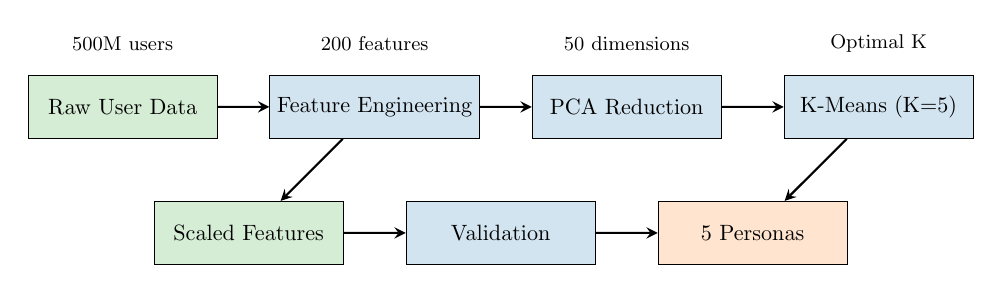
\begin{tikzpicture}[scale=0.8, transform shape]
\tikzstyle{process} = [rectangle, minimum width=3cm, minimum height=1cm, text centered, draw=black, fill=mlblue!20]
\tikzstyle{data} = [rectangle, minimum width=3cm, minimum height=1cm, text centered, draw=black, fill=mlgreen!20]
\tikzstyle{result} = [rectangle, minimum width=3cm, minimum height=1cm, text centered, draw=black, fill=mlorange!20]
\tikzstyle{arrow} = [thick,->,>=stealth]

% Pipeline
\node[data] (raw) at (0,3) {Raw User Data};
\node[process] (feature) at (4,3) {Feature Engineering};
\node[process] (pca) at (8,3) {PCA Reduction};
\node[process] (kmeans) at (12,3) {K-Means (K=5)};

\node[data] (scaled) at (2,1) {Scaled Features};
\node[process] (validate) at (6,1) {Validation};
\node[result] (segments) at (10,1) {5 Personas};

% Arrows
\draw[arrow] (raw) -- (feature);
\draw[arrow] (feature) -- (pca);
\draw[arrow] (pca) -- (kmeans);
\draw[arrow] (feature) -- (scaled);
\draw[arrow] (scaled) -- (validate);
\draw[arrow] (validate) -- (segments);
\draw[arrow] (kmeans) -- (segments);

% Annotations
\node at (0,4) {\small 500M users};
\node at (4,4) {\small 200 features};
\node at (8,4) {\small 50 dimensions};
\node at (12,4) {\small Optimal K};
\end{tikzpicture}

\vspace{1em}
\begin{columns}[T]
\begin{column}{0.3\textwidth}
\centering
\textbf{Processing Time}\\
\small 6 hours on cluster
\end{column}
\begin{column}{0.3\textwidth}
\centering
\textbf{Validation}\\
\small Silhouette: 0.68
\end{column}
\begin{column}{0.3\textwidth}
\centering
\textbf{Stability}\\
\small 92\% consistent
\end{column}
\end{columns}

\vspace{\fill}
\footnotesize\textcolor{mlgray}{Stability testing prevents fragile deployments - consistency across data variations separates robust patterns from statistical noise}
\end{frame}

% Discovered Personas
\begin{frame}{Step 3: The 5 Music Personas Discovered}
\begin{columns}[T]
\begin{column}{0.48\textwidth}
\textcolor{mlblue}{\Large\textbf{1. Loyalists (25\%)}}
\normalsize
• Replay favorite artists\\
• Low skip rate\\
• Deep catalogue diving\\
\vspace{0.5em}

\textcolor{mlorange}{\Large\textbf{2. Explorers (20\%)}}
\normalsize
• High discovery rate\\
• Diverse genres\\
• Early adopters\\
\vspace{0.5em}

\textcolor{mlgreen}{\Large\textbf{3. Casuals (30\%)}}
\normalsize
• Popular hits only\\
• Passive listening\\
• Radio-style consumption
\end{column}

\begin{column}{0.48\textwidth}
\textcolor{mlpurple}{\Large\textbf{4. Socialites (15\%)}}
\normalsize
• Share frequently\\
• Collaborative playlists\\
• Party music focus\\
\vspace{0.5em}

\textcolor{mlred}{\Large\textbf{5. Specialists (10\%)}}
\normalsize
• Single genre focus\\
• Deep expertise\\
• Curators \& tastemakers\\
\vspace{0.5em}

\begin{tcolorbox}[colback=mlyellow!20, colframe=mlorange!50]
\centering
\textbf{Key Discovery}\\
Behavior trumps demographics
\end{tcolorbox}
\end{column}
\end{columns}

\vspace{\fill}
\footnotesize\textcolor{mlgray}{Action-based segmentation surfaces latent needs - what users do reveals motivations demographic categories obscure}
\end{frame}

% Design Implementations
\begin{frame}{Step 4: Persona-Driven Features}
\centering
\Large\textbf{Tailored Experiences for Each Persona}
\normalsize
\vspace{0.5em}

\begin{tabular}{lccccc}
\toprule
\textbf{Feature} & \textbf{Loyalist} & \textbf{Explorer} & \textbf{Casual} & \textbf{Social} & \textbf{Specialist} \\
\midrule
Discover Weekly & Deep cuts & New artists & Top 40 & Viral hits & Niche gems \\
Home Screen & Artist focus & Genre mix & Simple & Social feed & Deep dive \\
Playlists & Artist radio & Discovery & Hits only & Collaborative & Genre pure \\
Notifications & New releases & New finds & Minimal & Friend activity & Genre news \\
Pricing & Premium & Premium+ & Free/Ad & Family plan & Curator tier \\
\bottomrule
\end{tabular}

\vspace{1em}
\begin{columns}[T]
\begin{column}{0.3\textwidth}
\centering
\includegraphics[width=0.8\textwidth]{charts/journey_comparison.pdf}\\
\small Loyalist Journey
\end{column}
\begin{column}{0.3\textwidth}
\centering
\includegraphics[width=0.8\textwidth]{charts/journey_comparison.pdf}\\
\small Explorer Journey
\end{column}
\begin{column}{0.3\textwidth}
\centering
\includegraphics[width=0.8\textwidth]{charts/journey_comparison.pdf}\\
\small Casual Journey
\end{column}
\end{columns}

\vspace{\fill}
\footnotesize\textcolor{mlgray}{Segmentation enables selective customization - identifying variation points allows targeted adaptation without complete product redesign}
\end{frame}

% Results and Impact
\begin{frame}{Results: The Power of Personalization}
\begin{columns}[T]
\begin{column}{0.55\textwidth}
\Large\textcolor{mlgreen}{\textbf{Quantitative Impact}}
\normalsize
\vspace{0.5em}

\begin{itemize}
\item \textbf{Engagement:} +40\% listening time
\item \textbf{Discovery:} +65\% new artist follows
\item \textbf{Retention:} +28\% monthly active users
\item \textbf{Revenue:} +31\% premium conversions
\item \textbf{NPS:} +35 points improvement
\end{itemize}

\vspace{0.5em}
\begin{tcolorbox}[colback=mlgreen!10, colframe=mlgreen!50]
\centering\Large\textbf{\$2.1B}\\
\normalsize Additional annual revenue
\end{tcolorbox}
\end{column}

\begin{column}{0.43\textwidth}
\Large\textcolor{mlpurple}{\textbf{Qualitative Impact}}
\normalsize
\vspace{0.5em}

\textbf{User Feedback:}\\
\small
``Finally, Spotify gets me!''\\
``Discover Weekly changed my life''\\
``It's like having a personal DJ''\\
\vspace{0.5em}

\textbf{Industry Recognition:}\\
• Best personalization (2023)\\
• Innovation award\\
• Case study at MIT\\
\vspace{0.5em}

\textcolor{mlblue}{\textbf{Competitive Advantage:}}\\
First-mover in ML personalization
\end{column}
\end{columns}

\vspace{\fill}
\footnotesize\textcolor{mlgray}{Measurable outcomes justify analytical investment - connecting segmentation to business metrics transforms clustering from exploration to strategy}
\end{frame}

% Practice Exercise
\begin{frame}{Your Turn: Practice Exercise}
\Large\textbf{Mini-Project: Segment Your App's Users}
\normalsize
\vspace{0.5em}

\begin{columns}[T]
\begin{column}{0.48\textwidth}
\textcolor{mlblue}{\textbf{Step 1: Data Preparation}}
\begin{enumerate}
\item Load user\_data.csv
\item Explore features
\item Scale the data
\item Check for outliers
\end{enumerate}

\vspace{0.5em}
\textcolor{mlorange}{\textbf{Step 2: Clustering}}
\begin{enumerate}
\item Try K = 3, 4, 5
\item Use elbow method
\item Calculate silhouette
\item Choose optimal K
\end{enumerate}
\end{column}

\begin{column}{0.48\textwidth}
\textcolor{mlgreen}{\textbf{Step 3: Analysis}}
\begin{enumerate}
\item Profile each cluster
\item Name your personas
\item Identify key differences
\item Find opportunities
\end{enumerate}

\vspace{0.5em}
\textcolor{mlpurple}{\textbf{Step 4: Design}}
\begin{enumerate}
\item Create empathy map
\item Design features
\item Propose UI changes
\item Present findings
\end{enumerate}
\end{column}
\end{columns}

\vspace{0.5em}
\begin{tcolorbox}[colback=mlyellow!20, colframe=mlorange!50]
\centering
\textbf{Deliverable:} 5-slide presentation with your personas and recommendations\\
\textbf{Time:} 45 minutes | \textbf{Tools:} Python, sklearn, matplotlib
\end{tcolorbox}

\vspace{\fill}
\footnotesize\textcolor{mlgray}{Structured workflows reduce cognitive load - systematic processes enable focus on insights rather than mechanics during analysis}
\end{frame}

% Key Takeaways
\begin{frame}{Key Takeaways: Clustering for Empathy}
\begin{columns}[T]
\begin{column}{0.48\textwidth}
\Large\textcolor{mlblue}{\textbf{Technical Lessons}}
\normalsize
\vspace{0.5em}
\begin{enumerate}
\item Always scale your features
\item Validate with multiple methods
\item Start simple (K-means)
\item Consider your data shape
\item Test stability
\end{enumerate}

\vspace{0.5em}
\begin{tcolorbox}[colback=mlblue!10, colframe=mlblue!50]
\centering
\textbf{Remember:}\\
No clustering is perfect,\\but all reveal insights
\end{tcolorbox}
\end{column}

\begin{column}{0.48\textwidth}
\Large\textcolor{mlpurple}{\textbf{Design Lessons}}
\normalsize
\vspace{0.5em}
\begin{enumerate}
\item Clusters $\neq$ demographics
\item Behavior reveals needs
\item Each segment is valuable
\item Personalization scales
\item Test with real users
\end{enumerate}

\vspace{0.5em}
\begin{tcolorbox}[colback=mlpurple!10, colframe=mlpurple!50]
\centering
\textbf{Remember:}\\
Data augments empathy,\\doesn't replace it
\end{tcolorbox}
\end{column}
\end{columns}

\vspace{0.5em}
\begin{center}
\Large\textcolor{mlgreen}{\textbf{You now have the power to understand millions of users!}}
\end{center}

\vspace{\fill}
\footnotesize\textcolor{mlgray}{Technical capability without design thinking yields unused tools - integration of analytical methods with human understanding creates actionable innovation}
\end{frame}
% APPENDIX: TECHNICAL DEEP DIVE
\appendix
\section{Technical Appendix}

% Appendix Slide 1: K-Means Mathematics
\begin{frame}
\frametitle{\Large Appendix: K-Means Mathematics (Optional)}
\framesubtitle{The Mathematical Foundation - For Those Interested}

\Large\textbf{What K-means tries to minimize:}
\normalsize
$$J = \sum_{i=1}^{n} \sum_{j=1}^{k} w_{ij} ||x_i - \mu_j||^2$$

\textit{In simple terms: Make points close to their group centers}

Where:
\begin{itemize}
\item $n$ = number of data points
\vspace{0.3em}
\item $k$ = number of clusters
\vspace{0.3em}
\item $w_{ij}$ = 1 if $x_i$ belongs to cluster $j$, 0 otherwise
\vspace{0.3em}
\item $\mu_j$ = centroid of cluster $j$
\end{itemize}

\vspace{0.5em}
\Large\textbf{Update Rules:}
\normalsize
\begin{enumerate}
\item Assignment: $c^{(i)} = \arg\min_j ||x^{(i)} - \mu_j||^2$
\item Update: $\mu_j = \frac{1}{|S_j|} \sum_{i \in S_j} x^{(i)}$
\end{enumerate}
\end{frame}

% Appendix Slide 2: Distance Metrics Formulas
\begin{frame}
\frametitle{\Large Appendix: Distance Metrics (Optional)}
\framesubtitle{Different Ways to Measure "How Far Apart" Things Are}

\begin{columns}[T]
\begin{column}{0.48\textwidth}
\textbf{Euclidean Distance:}
$$d(x,y) = \sqrt{\sum_{i=1}^{n} (x_i - y_i)^2}$$

\vspace{0.5em}
\textbf{Manhattan Distance:}
$$d(x,y) = \sum_{i=1}^{n} |x_i - y_i|$$

\vspace{0.5em}
\textbf{Minkowski Distance:}
$$d(x,y) = \left(\sum_{i=1}^{n} |x_i - y_i|^p\right)^{1/p}$$
\end{column}

\begin{column}{0.48\textwidth}
\textbf{Cosine Similarity:}
$$\cos(\theta) = \frac{x \cdot y}{||x|| \cdot ||y||}$$

\vspace{0.5em}
\textbf{Jaccard Distance:}
$$J(A,B) = 1 - \frac{|A \cap B|}{|A \cup B|}$$

\vspace{0.5em}
\textbf{Mahalanobis Distance:}
$$d(x,y) = \sqrt{(x-y)^T S^{-1} (x-y)}$$
\end{column}
\end{columns}
\end{frame}

% Appendix Slide 3: Silhouette Coefficient
\begin{frame}
\frametitle{\Large Appendix: Silhouette Score Explained}
\framesubtitle{How We Know If Groups Are Good}

\Large\textbf{Silhouette Score for point $i$:}
\normalsize
$$s(i) = \frac{b(i) - a(i)}{\max\{a(i), b(i)\}}$$

Where:
\begin{itemize}
\item $a(i)$ = average distance to points in same cluster
\vspace{0.3em}
\item $b(i)$ = average distance to points in nearest neighbor cluster
\end{itemize}

\vspace{0.5em}
\Large\textbf{Interpretation:}
\normalsize
\begin{itemize}
\item $s(i) \approx 1$: Well clustered
\vspace{0.3em}
\item $s(i) \approx 0$: On border between clusters
\vspace{0.3em}
\item $s(i) \approx -1$: Misclassified
\end{itemize}

\vspace{0.5em}
\Large\textbf{Overall Score:}
\normalsize
$$S = \frac{1}{n} \sum_{i=1}^{n} s(i)$$
\end{frame}

% Appendix Slide 4: PCA for Visualization
\begin{frame}
\frametitle{\Large Appendix: Visualizing High-Dimensional Data}
\framesubtitle{Making Complex Data Viewable in 2D}

\begin{columns}[T]
\begin{column}{0.55\textwidth}
\begin{center}
\includegraphics[width=\textwidth]{charts/pca_clusters.pdf}
\end{center}
\end{column}

\begin{column}{0.43\textwidth}
\Large\textbf{PCA Process:}
\normalsize
\begin{enumerate}
\item Standardize data
\vspace{0.3em}
\item Compute covariance matrix
\vspace{0.3em}
\item Find eigenvectors/values
\vspace{0.3em}
\item Select top 2 components
\vspace{0.3em}
\item Transform data
\end{enumerate}

\vspace{0.5em}
\textbf{Variance Explained:}
\begin{itemize}
\item PC1: 45.2\%
\vspace{0.3em}
\item PC2: 28.7\%
\vspace{0.3em}
\item Total: 73.9\%
\end{itemize}
\end{column}
\end{columns}
\end{frame}

% NEW: t-SNE vs PCA Comparison
\begin{frame}
\frametitle{\Large Dimensionality Reduction: PCA vs t-SNE}
\framesubtitle{Revealing Hidden Patterns in High-Dimensional Innovation Space}

\begin{center}
\includegraphics[width=0.85\textwidth]{charts/tsne_pca_comparison.pdf}
\end{center}
\end{frame}

% Appendix Slide 5: DBSCAN Algorithm
\begin{frame}
\frametitle{\Large Appendix: How DBSCAN Works}
\framesubtitle{Finding Groups Based on How Close Points Are}

\Large\textbf{Key Parameters:}
\normalsize
\begin{itemize}
\item $\epsilon$ (eps): Maximum distance between points
\vspace{0.3em}
\item MinPts: Minimum points to form dense region
\end{itemize}

\vspace{0.5em}
\Large\textbf{Point Classification:}
\normalsize
\begin{itemize}
\item \textbf{Core point}: Has $\geq$ MinPts within $\epsilon$
\vspace{0.3em}
\item \textbf{Border point}: Within $\epsilon$ of core point
\vspace{0.3em}
\item \textbf{Noise point}: Neither core nor border
\end{itemize}

\vspace{0.5em}
\Large\textbf{Algorithm Steps:}
\normalsize
\begin{enumerate}
\item Find all core points
\vspace{0.3em}
\item Form clusters from core points within $\epsilon$
\vspace{0.3em}
\item Assign border points to clusters
\vspace{0.3em}
\item Mark remaining as noise
\end{enumerate}
\end{frame}

% NEW: DBSCAN Parameter Tuning
\begin{frame}
\frametitle{\Large DBSCAN Parameter Tuning}
\framesubtitle{Impact of eps and min\_samples on Clustering Results}

\begin{center}
\includegraphics[width=0.85\textwidth]{charts/dbscan_tuning.pdf}
\end{center}
\end{frame}

% Appendix Slide 6: Python Code Examples
\begin{frame}[fragile]
\frametitle{\Large Appendix: Python Implementation}
\framesubtitle{Ready-to-Use Code Snippets}

\begin{columns}[T]
\begin{column}{0.48\textwidth}
\begin{tcolorbox}[colback=gray!5, colframe=mlblue!50, title={\small K-Means Clustering}]
\begin{lstlisting}[basicstyle=\scriptsize\ttfamily]
from sklearn.cluster import KMeans
import numpy as np

# Generate sample data
X = np.random.randn(1000, 2)

# Configure and fit K-means
kmeans = KMeans(
    n_clusters=3,
    random_state=42,
    n_init=10
)
labels = kmeans.fit_predict(X)

# Get cluster centers
centers = kmeans.cluster_centers_

# Calculate inertia
inertia = kmeans.inertia_
\end{lstlisting}
\end{tcolorbox}
\end{column}

\begin{column}{0.48\textwidth}
\begin{tcolorbox}[colback=gray!5, colframe=mlorange!50, title={\small DBSCAN Clustering}]
\begin{lstlisting}[basicstyle=\scriptsize\ttfamily]
from sklearn.cluster import DBSCAN

# Configure DBSCAN
dbscan = DBSCAN(
    eps=0.3,
    min_samples=5,
    metric='euclidean'
)

# Fit and predict
labels = dbscan.fit_predict(X)

# Analyze results
outliers = labels == -1
n_clusters = len(set(labels)) - 1

print(f"Clusters: {n_clusters}")
print(f"Outliers: {sum(outliers)}")
print(f"Coverage: {100*(1-sum(outliers)/len(labels)):.1f}%")
\end{lstlisting}
\end{tcolorbox}
\end{column}
\end{columns}
\end{frame}

% NEW: Code Example for Evaluation
\begin{frame}[fragile]
\frametitle{\Large Appendix: Evaluation Metrics Code}
\framesubtitle{Measuring Clustering Quality}

\begin{columns}[T]
\begin{column}{0.48\textwidth}
\begin{tcolorbox}[colback=gray!5, colframe=mlgreen!50, title={\small Silhouette Analysis}]
\begin{lstlisting}[basicstyle=\scriptsize\ttfamily]
from sklearn.metrics import silhouette_score
from sklearn.metrics import silhouette_samples

# Calculate overall score
score = silhouette_score(X, labels)
print(f"Silhouette Score: {score:.3f}")

# Per-sample scores
sample_scores = silhouette_samples(X, labels)

# Per-cluster average
for i in range(n_clusters):
    cluster_scores = sample_scores[labels == i]
    avg = cluster_scores.mean()
    print(f"Cluster {i}: {avg:.3f}")
\end{lstlisting}
\end{tcolorbox}
\end{column}

\begin{column}{0.48\textwidth}
\begin{tcolorbox}[colback=gray!5, colframe=mlpurple!50, title={\small Finding Optimal K}]
\begin{lstlisting}[basicstyle=\scriptsize\ttfamily]
# Elbow method
inertias = []
silhouettes = []
K_range = range(2, 10)

for k in K_range:
    km = KMeans(n_clusters=k,
                random_state=42)
    labels = km.fit_predict(X)
    
    inertias.append(km.inertia_)
    silhouettes.append(
        silhouette_score(X, labels)
    )

# Find elbow point
# Plot inertias vs K
# Choose K at elbow
\end{lstlisting}
\end{tcolorbox}
\end{column}
\end{columns}
\end{frame}

% Appendix Slide 7: Implementation Hints
\begin{frame}
\frametitle{\Large Appendix: Implementation Guidelines}
\framesubtitle{Practical Considerations}

\begin{columns}[T]
\begin{column}{0.48\textwidth}
\begin{tcolorbox}[colback=mlblue!10, colframe=mlblue!50, title=Data Preparation]
\normalsize
\begin{itemize}
\item Standardize features
\item Handle missing values
\item Remove outliers (if needed)
\item Feature selection/engineering
\item Consider scaling methods
\end{itemize}
\end{tcolorbox}

\vspace{0.5em}
\begin{tcolorbox}[colback=mlgreen!10, colframe=mlgreen!50, title=Algorithm Selection]
\normalsize
\begin{itemize}
\item K-means: Spherical, similar size
\item DBSCAN: Arbitrary shapes
\item Hierarchical: Nested structure
\item GMM: Overlapping clusters
\end{itemize}
\end{tcolorbox}
\end{column}

\begin{column}{0.48\textwidth}
\begin{tcolorbox}[colback=mlorange!10, colframe=mlorange!50, title=Validation Methods]
\normalsize
\begin{itemize}
\item Silhouette score
\item Davies-Bouldin index
\item Calinski-Harabasz score
\item Visual inspection
\item Domain expert review
\end{itemize}
\end{tcolorbox}

\vspace{0.5em}
\begin{tcolorbox}[colback=mlred!10, colframe=mlred!50, title=Common Pitfalls]
\normalsize
\begin{itemize}
\item Not scaling features
\item Wrong distance metric
\item Ignoring outliers
\item Over-clustering
\item Forcing clusters
\end{itemize}
\end{tcolorbox}
\end{column}
\end{columns}
\end{frame}

% NEW: Glossary of Technical Terms
\begin{frame}
\frametitle{\Large Glossary of Technical Terms}
\framesubtitle{Key Concepts Reference}

\begin{columns}[T]
\begin{column}{0.48\textwidth}
\small
\textbf{Algorithms:}
\begin{itemize}
\item \textbf{K-means}: Partitions data into K spherical clusters
\item \textbf{DBSCAN}: Density-based clustering for arbitrary shapes
\item \textbf{GMM}: Gaussian Mixture Models for soft clustering
\item \textbf{Hierarchical}: Tree-based clustering approach
\end{itemize}

\vspace{0.5em}
\textbf{Metrics:}
\begin{itemize}
\item \textbf{Silhouette}: Measures cluster separation (-1 to 1)
\item \textbf{Inertia}: Sum of squared distances to centroids
\item \textbf{Davies-Bouldin}: Ratio of within to between cluster distance
\end{itemize}
\end{column}

\begin{column}{0.48\textwidth}
\small
\textbf{Concepts:}
\begin{itemize}
\item \textbf{Centroid}: Center point of a cluster
\item \textbf{Elbow Method}: Technique to find optimal K
\item \textbf{Outlier}: Data point not belonging to any cluster
\item \textbf{Convergence}: When algorithm stops improving
\end{itemize}

\vspace{0.5em}
\textbf{Preprocessing:}
\begin{itemize}
\item \textbf{Standardization}: Zero mean, unit variance
\item \textbf{Normalization}: Scale to [0,1] range
\item \textbf{PCA}: Principal Component Analysis
\item \textbf{t-SNE}: t-distributed Stochastic Neighbor Embedding
\end{itemize}
\end{column}
\end{columns}
\end{frame}

\end{document}